%%%%%%%%%%%%%%%%%%%%%%%%%%%%%%%%%%%%%%%%%%%%%%%%%%%%%%%%%%%%%%%%%%%%%%%%%%%%%%%%
%% Plantilla de memoria en LaTeX para la ETSIT - Universidad Rey Juan Carlos
%%
%% Por Gregorio Robles <grex arroba gsyc.urjc.es>
%%     Grupo de Sistemas y Comunicaciones
%%     Escuela Técnica Superior de Ingenieros de Telecomunicación
%%     Universidad Rey Juan Carlos
%% (muchas ideas tomadas de Internet, colegas del GSyC, antiguos alumnos...
%%  etc. Muchas gracias a todos)
%%
%% La última versión de esta plantilla está siempre disponible en:
%%     https://github.com/gregoriorobles/plantilla-memoria
%%
%% Para obtener PDF, ejecuta en la shell:
%%   make
%% (las imágenes deben ir en PNG o JPG)

%%%%%%%%%%%%%%%%%%%%%%%%%%%%%%%%%%%%%%%%%%%%%%%%%%%%%%%%%%%%%%%%%%%%%%%%%%%%%%%%

\documentclass[a4paper, 12pt]{book}
%\usepackage[T1]{fontenc}

\usepackage[a4paper, left=2.5cm, right=2.5cm, top=3cm, bottom=3cm]{geometry}
\usepackage{times}
\usepackage[utf8]{inputenc}
\usepackage[spanish]{babel} % Comenta esta línea si tu memoria es en inglés
\usepackage{url}
%\usepackage[dvipdfm]{graphicx}
\usepackage{graphicx}
\usepackage{float}  %% H para posicionar figuras
\usepackage[nottoc, notlot, notlof, notindex]{tocbibind} %% Opciones de índice
\usepackage{latexsym}  %% Logo LaTeX
\usepackage{listings}

\title{Memoria del Proyecto}
\author{Nombre del autor}

\renewcommand{\baselinestretch}{1.5}  %% Interlineado

\begin{document}

\renewcommand{\refname}{Bibliografía}  %% Renombrando
\renewcommand{\appendixname}{Apéndice}

%%%%%%%%%%%%%%%%%%%%%%%%%%%%%%%%%%%%%%%%%%%%%%%%%%%%%%%%%%%%%%%%%%%%%%%%%%%%%%%%
% PORTADA

\begin{titlepage}
\begin{center}
\begin{tabular}[c]{c c}
%\includegraphics[bb=0 0 194 352, scale=0.25]{logo} &
\includegraphics[scale=0.25]{img/logo_vect.png} &
\begin{tabular}[b]{l}
\Huge
\textsf{UNIVERSIDAD} \\
\Huge
\textsf{REY JUAN CARLOS} \\
\end{tabular}
\\
\end{tabular}

\vspace{3cm}

\Large
MÁSTER DE INGENIERÍA DE TELECOMUNICACIÓN

\vspace{0.4cm}

\large
Curso Académico 2018/2019

\vspace{0.8cm}

Trabajo Fin de Máster

\vspace{2.5cm}

\LARGE
ANÁLISIS Y ESTUDIO DEL USO DE \textit{PYTHONIC IDIOMS}

\vspace{4cm}

\large
Autor : José Javier Merchante \\
Tutor : Dr. Gregorio Robles
\end{center}
\end{titlepage}

\newpage
\mbox{}
\thispagestyle{empty} % para que no se numere esta pagina


%%%%%%%%%%%%%%%%%%%%%%%%%%%%%%%%%%%%%%%%%%%%%%%%%%%%%%%%%%%%%%%%%%%%%%%%%%%%%%%%
%%%% Para firmar
\clearpage
\pagenumbering{gobble}
\chapter*{}

\vspace{-4cm}
\begin{center}
\LARGE
\textbf{Trabajo Fin de Máster}

\vspace{1cm}
\large
Análisis y Estudio del Uso de \textit{Pythonic Idioms}

\vspace{1cm}
\large
\textbf{Autor :} José Javier Merchante \\
\textbf{Tutor :} Dr. Gregorio Robles Martínez

\end{center}

\vspace{1cm}
La defensa del presente Proyecto Fin de Carrera se realizó el día \qquad$\;\,$ de \qquad\qquad\qquad\qquad \newline de 2019, siendo calificada por el siguiente tribunal:


\vspace{0.5cm}
\textbf{Presidente:}

\vspace{1.2cm}
\textbf{Secretario:}

\vspace{1.2cm}
\textbf{Vocal:}


\vspace{1.2cm}
y habiendo obtenido la siguiente calificación:

\vspace{1cm}
\textbf{Calificación:}


\vspace{1cm}
\begin{flushright}
Fuenlabrada, a \qquad$\;\,$ de \qquad\qquad\qquad\qquad de 2019
\end{flushright}

%%%%%%%%%%%%%%%%%%%%%%%%%%%%%%%%%%%%%%%%%%%%%%%%%%%%%%%%%%%%%%%%%%%%%%%%%%%%%%%%
%%%% Dedicatoria

\chapter*{}
\pagenumbering{Roman} % para comenzar la numeracion de paginas en numeros romanos
\begin{flushright}
\textit{Dedicado a \\
mis padres y mi hermana}
\end{flushright}

%%%%%%%%%%%%%%%%%%%%%%%%%%%%%%%%%%%%%%%%%%%%%%%%%%%%%%%%%%%%%%%%%%%%%%%%%%%%%%%%
%%%% Agradecimientos

\chapter*{Agradecimientos}
%\addcontentsline{toc}{chapter}{Agradecimientos} % si queremos que aparezca en el índice
\markboth{AGRADECIMIENTOS}{AGRADECIMIENTOS} % encabezado 

La realización de este trabajo de fin de máster supone el final de una gran etapa de mi vida. Se queda grabados recuerdos de estrés, de aprobados ajustados y matrículas de honor tras tanto tiempo dedicado a cada una de las asignaturas. Los momentos en los que la compaginación de trabajo y estudios no eran tan sencillos como la gente afirmaba.

Todo este esfuerzo, por fortuna, no lo he realizado solo, sino que la compañía siempre ha sido una clara aliada, con un apoyo constante que al final ha dado sus frutos.

Es por ello que quiero agradecer a mi familia, por esos momentos en los que estuvieron preocupándose por mi, animándome a continuar cuando las circunstancias no eran los mejores, y alegrándose por cada una de las metas que juntos hemos conseguido.

También agradecer a mis compañeros de clase por todo este tiempo compartido juntos, estando unidos como una pequeña familia, tanto para lo bueno como para lo malo, y con ese ``pique'' constante por buscar siempre la mejor nota de la clase.

Por último, y no menos importante, agradecer a Gregorio estos años que tanta experiencia que me ha aportado. Tanto en el pasado de manera curricular, como trabajando junto a él, así como en lo personal. Siempre ha creído y confiado en mí, y ha buscado continuamente un ``JJ'' que estuviera en lo más alto, gracias.

A todos ellos les debo este paso en mi vida, ¡gracias!

%%%%%%%%%%%%%%%%%%%%%%%%%%%%%%%%%%%%%%%%%%%%%%%%%%%%%%%%%%%%%%%%%%%%%%%%%%%%%%%%
%%%% Resumen

\chapter*{Resumen}
%\addcontentsline{toc}{chapter}{Resumen} % si queremos que aparezca en el índice
\markboth{RESUMEN}{RESUMEN} % encabezado

En este proyecto se realiza un estudio acerca de los elementos avanzados del lenguaje de programación Python.

Para el desarrollo del mismo, se han realizado entrevistas a programadores para conocer su percepción acerca del significado y aplicación de estas estructuras \textit{pythonic}. A partir de los resultados, se han podido obtener unas conclusiones precisas que podrán ser de utilidad para estudios relacionados y que demuestra la importancia del proyecto que se está realizando.

Por otro lado, se ha realizado la implementación para el análisis de repositorios escritos en Python. Cualquier programador, tanto experto como principiante, puede realizar un análisis de sus repositorios mediante una herramienta web, y obtener unos resultados acerca de los mismos para mejorar en el ámbito de Python.

Este proyecto se enmarca en un trabajo de investigación para la identificación y conocimiento de la cultura de uno de los lenguajes de programación más usados hoy en día. Se busca mejorar la comprensión del término \textit{pythonic} así como incentivar el uso de dichas estructuras. 



%%%%%%%%%%%%%%%%%%%%%%%%%%%%%%%%%%%%%%%%%%%%%%%%%%%%%%%%%%%%%%%%%%%%%%%%%%%%%%%%
%%%% Resumen en inglés

\chapter*{Summary}
%\addcontentsline{toc}{chapter}{Summary} % si queremos que aparezca en el índice
\markboth{SUMMARY}{SUMMARY} % encabezado

This project is a study about \textit{Pythonic idioms}.

Interviews to programmers have been conducted in order to gather information about the knowledge and application of \textit{pythonic idioms}. Based on the results, it has been possible to obtain some conlusions that can be used for related studies, and shows the importance of the project that is being carried out.

On the other hand, we have made a implementation for the analysis of Python repositories. Any programer, both expert and beginner, can perform an anlysis of their repositories though a web tool and obtain some results about them to improve in the field of Python.

This project is part of a research work of one of the most important languages used today. The aim is to improve the understanding of the term \textit{pythonic}, as well as to encourage the use of these structures.

%%%%%%%%%%%%%%%%%%%%%%%%%%%%%%%%%%%%%%%%%%%%%%%%%%%%%%%%%%%%%%%%%%%%%%%%%%%%%%%%
%%%%%%%%%%%%%%%%%%%%%%%%%%%%%%%%%%%%%%%%%%%%%%%%%%%%%%%%%%%%%%%%%%%%%%%%%%%%%%%%
% ÍNDICES %
%%%%%%%%%%%%%%%%%%%%%%%%%%%%%%%%%%%%%%%%%%%%%%%%%%%%%%%%%%%%%%%%%%%%%%%%%%%%%%%%

% Las buenas noticias es que los índices se generan automáticamente.
% Lo único que tienes que hacer es elegir cuáles quieren que se generen,
% y comentar/descomentar esa instrucción de LaTeX.

%%%% Índice de contenidos
\tableofcontents 
%%%% Índice de figuras
\cleardoublepage
%\addcontentsline{toc}{chapter}{Lista de figuras} % para que aparezca en el indice de contenidos
\listoffigures % indice de figuras
%%%% Índice de tablas
%\cleardoublepage
%\addcontentsline{toc}{chapter}{Lista de tablas} % para que aparezca en el indice de contenidos
%\listoftables % indice de tablas


%%%%%%%%%%%%%%%%%%%%%%%%%%%%%%%%%%%%%%%%%%%%%%%%%%%%%%%%%%%%%%%%%%%%%%%%%%%%%%%%
%%%%%%%%%%%%%%%%%%%%%%%%%%%%%%%%%%%%%%%%%%%%%%%%%%%%%%%%%%%%%%%%%%%%%%%%%%%%%%%%
% INTRODUCCIÓN %
%%%%%%%%%%%%%%%%%%%%%%%%%%%%%%%%%%%%%%%%%%%%%%%%%%%%%%%%%%%%%%%%%%%%%%%%%%%%%%%%

\cleardoublepage

\chapter{Introducción}
\label{chap:intro}
\pagenumbering{arabic}

En la era en la que vivimos, en múltiples disciplinas y sobre todo enfocados en el ámbito de la telecomunicación, el manejo de la información es un pilar clave. El uso de la programación para el análisis de los datos es imprescindible para poder filtrar y generar nueva información que podría ser de más utilidad.

En la actualidad, la cantidad de código escrito por programadores de diferentes ámbitos aumenta considerablemente. Desde crear nuevos programas que faciliten la realización de determinadas tareas de cualquier trabajador, hasta herramientas enfocadas en el análisis de datos para conocer la evolución de un producto.

La importancia de mantener el código ``limpio'', es decir, siguiendo unos determinados patrones de diseño, es bastante determinante para poder ser mantenido para solucionar futuros errores o incluso implementar nuevas características.

La evolución de los proyectos almacenados en plataformas de desarrollo colaborativo, como puede ser el caso de GitHub o GitLab entre otros, aumenta significativamente, tanto en número, como en el contenido de los mismos.

La relevancia del \textit{Open Source} (código que está disponible públicamente bajo unas condiciones determinadas que permiten copiar, modificar y redistribuir el software) ha ido cobrando mayor importancia a lo largo de los último años. Las grandes compañías cada vez optan más por publicar su software, aunque sólo sea de algunas aplicaciones, como en el caso de \textit{Microsoft}.

La publicación de código en abierto supone un esfuerzo adicional por parte de las organizaciones que lo mantienen. El código siempre debe mantenerse \textit{limpio}, es decir, seguir unos determinados patrones de diseño para poder ser mantenido para futuros errores, pero además,  si las compañías quieren beneficiarse de uno de los beneficios del código abierto, como es el caso de contribución externa al proyecto, es importante reflejar una buena imagen del código.

Es por cuestiones como las mencionadas, que se hace necesario el uso de herramientas que puedan ayudar o facilitar este tipo de tareas. En el presente proyecto vamos a poner el foco en uno de los lenguajes más populares en los último años, Python. En el momento de escribir esta memoria, se encuentra el tercero en el índice TIOBE\footnote{https://www.tiobe.com/tiobe-index/}, y es uno de los lenguajes que más ha crecido en los últimos años.

Este lenguaje tiene a su disposición un gran número de herramientas como es el caso de \textit{pep8} o \textit{pylint} que ayudan a seguir una serie de convenios en la sintaxis. Sin embargo, nosotros queremos hacer un estudio que vaya más allá de las reglas del estilo y enfocarlo más a las estructuras utilizadas.

El uso de determinadas elementos denominados \textit{idioms}, facilitan en gran medida la programación en un lenguaje, y por lo tanto, el aprendizaje y aplicación de los mismos favorecen a un código más limpio, más sencillo de leer, e incluso en algunos casos, mejora el rendimiento de la ejecución al ser estructuras más optimizadas.

\section{Conceptos previos}
\label{sec:ConceptosPrevios}


\section{Motivación}
\label{sec:motivacion}

En la actualidad, tal y como se comentó anteriormente, se hace necesario un estudio para mejorar el estado del código de muchos programadores. Existen cantidad de ellos que por exigencias personales o incluso por necesidades de las empresa necesitan enriquecer su código.

Para ilustrar un ejemplo sencillo, un programador principiante en Python, y que quizá tiene más experiencia en otros lenguajes, podría programar el siguiente extracto de código:

\begin{lstlisting}[language=Python, basicstyle=\small]
positions = ['Ana', 'Juan', 'Pepe', 'Marta']
i = 0
for name in positions:
    i += 1
    print(i, name)
    
\end{lstlisting}
Se puede observar una iteración sobre una lista, y mediante una variable auxiliar, imprime por pantalla las posiciones en las que han quedado unos corredores. Este código ejecuta a la perfección, hace su labor y sigue las reglas de estilo en Python. Sin embargo, existe una manera más ``bonita'' y eficiente de hacerlo, que es lo que sería considera por la comunidad un código más \textit{pythonic}:

\begin{lstlisting}[language=Python, basicstyle=\small]
positions = ['Ana', 'Juan', 'Pepe', 'Marta']
for i, name in enumerate(positions, 1):
    print(i, name)
\end{lstlisting}

Tal y como puede observarse, el número de líneas ahora es menor, es más sencillo de leer, y además, se puede comprobar que con un bucle de una lista de mayores dimensiones se mejora el tiempo de ejecución del programa.

Por lo tanto, la necesidad de aplicaciones que nos permitan conocer este tipo de estructuras o identificar cambios en nuestro código puede ser de gran ayuda tanto a programadores principiantes como a aquellos que quieran conocer más acerca del lenguaje.

Recurrir a varios libros y páginas webs para leer con todo este contenido siempre es una opción válida, pero conocer nuestros errores mientras programamos o conocer nuevas estructuras agrupadas en una única web puede ser siempre una manera más útil de aprender.

\section{Contexto}
\label{contexto}

Como contexto de este Trabajo de Fin de Máster se encuentra el desarrollo de una herramienta de búsqueda de \textit{idioms}, la publicación de pequeños artículos en seminarios internaciones, participación en la PyConES como ponente y la colaboración con la universidad de Zúrich para la publicación un artículo en una conferencia.

El programa para la identificación de \textit{pythonic idioms} se desarrolló para un Trabajo de Fin de Grado. El autor y el director fueron los mismos que para el presente proyecto. Para la realización de la aplicación se generó una lista de en torno a 100 \textit{idioms} documentándose a partir de diferentes libros, sitios web, foros, e incluso por experiencias personales. La herramienta consistía en un \textit{script} de Python que seguía el siguiente guión:
\begin{itemize}
    \item El usuario introducía en la llamada un repositorio \textit{git}.
    \item El programa se encargaba de clonar el repositorio en local para obtener el código.
    \item Posteriormente se identificaban y seleccionaban los ficheros que fueran Python, es decir, terminados en \textit{.py}, o sin extensión y la primera línea (\textit{shebang}) indique que es un fichero Python.
    \item Por cada uno de los ficheros, se dividía el código en \textit{tokens} con el \textit{lexer} de la librería \textit{Pygments} (un resaltador de sintaxis).
    \item Se recorría la cadena de \textit{tokens} y se identificaban cada uno de los \textit{idioms}. En unos casos eran simples al ser llamadas a funciones, y en otros casos se buscaban determinados patrones.
    \item Por cada uno de los \textit{idioms} encontrados se almacenaba la línea y fichero donde se habían encontrado y además se intentaba identificar el autor del mismo. Para ello se miraba con \textit{git blame} el correo de la última persona que había modificado la línea.
    \item Finalmente se ofrecían al usuario todos los \textit{idioms} identificados.
\end{itemize}

Este programa ha servido de base para la realización de la aplicación web con alguna modificación para adaptarlo a la recogida de los datos.

Por otro lado, es importante señalar la colaboración con profesores y un estudiante de doctorado de la Universidad de Zúrich. Junto a ellos, se elaboró una publicación de un artículo en una conferencia. En dicho artículo, se realiza un análisis de cómo los programadores entienden el término \textit{pythonic} a partir de entrevistas, se muestra un catálogo de \textit{idioms} a partir de la literatura y se exponen los efectos de tener en un lenguaje un término específico para la calidad del código, considerando el potencial que podría tener para otros lenguajes y ecosistemas~\cite{pythononroad}.

Cabe mencionar en el contexto de este trabajo, la participación en pequeños seminarios internacionales de software enfocados a presentar el trabajo en progreso. Estos seminarios fueron SATToSE\footnote{http://sattose.org/} y BENEVOL\footnote{http://ansymore.uantwerpen.be/benevol-2017-agenda, https://benevol2016.wordpress.com/program/}. Se enfocaban principalmente en presentaciones o artículos relacionados con las técnicas y herramientas para la evolución del código.

Finalmente destacar que se realizó la presentación de la herramienta web para el análisis de repositorios en la PyConES, la conferencia Python más grande de ámbito nacional, a partir de la cual se obtuvieron candidatos para la realización de entrevistas acerca del código \textit{pythonic}.

\section{Estructura de la memoria}
\label{sec:Estructura}
En esta sección se detalla la estructura en la que se ordena la presente memoria para facilitar su comprensión:
\begin{itemize}

    \item En la introducción del capítulo \ref{chap:intro} se realiza una descripción del proyecto incluyendo algunos conceptos claves, mostrando la motivación adherida al trabajo y exponiendo el contexto derivado del estudio.

    \item En el capítulo \ref{chap:objetivos} se encuentran los objetivos, generales y específicos, que se intentan abordar en este trabajo.

    \item A continuación en el capítulo \ref{chap:arte} se mostrarán las tecnologías utilizadas en el proyecto y una breve pero explicativa descripción de las mismas.

    \item Situado en el capítulo \ref{chap:cualitativo} se explica la realización de las entrevistas. Se enumeran las categorías de preguntas que se han realizado, y los resultados obtenidos de las mismas.

    \item Por otro lado, en el capitulo \ref{chap:cuantitativo} se realiza un explicación extensa del uso de la aplicación web de análisis de repositorios.
    
    \item Tras la explicación de lo anterior, en el capítulo \ref{chap:conclusiones} se muestran las conclusiones finales del proyecto, objetivos alcanzados y una breve valoración personal.
    
\end{itemize}
%%%%%%%%%%%%%%%%%%%%%%%%%%%%%%%%%%%%%%%%%%%%%%%%%%%%%%%%%%%%%%%%%%%%%%%%%%%%%%%%
%%%%%%%%%%%%%%%%%%%%%%%%%%%%%%%%%%%%%%%%%%%%%%%%%%%%%%%%%%%%%%%%%%%%%%%%%%%%%%%%
% OBJETIVOS %
%%%%%%%%%%%%%%%%%%%%%%%%%%%%%%%%%%%%%%%%%%%%%%%%%%%%%%%%%%%%%%%%%%%%%%%%%%%%%%%%

\cleardoublepage % empezamos en página impar
\chapter{Objetivos} % título del capítulo (se muestra)
\label{chap:objetivos} % identificador del capítulo (no se muestra, es para poder referenciarlo)

\section{Objetivo general} % título de sección (se muestra)
\label{sec:objetivo-general} % identificador de sección (no se muestra, es para poder referenciarla)

El objetivo principal de esta memoria es conocer la importancia de escribir código limpio en los programas. Dentro de la comunidad de Python se destaca siempre el código \textit{pythonic}, es por ello que hemos querido profundizar y conocer los diferentes aspectos que son de más relevancia.

Se pretende dar respuestas a preguntas como:

\begin{itemize}
    \item ¿Qué son según la comunidad los elementos \textit{pythonic}?
    \item ¿Qué importancia tienen en las empresas y en plataformas de software colaborativo?
    \item ¿Cuál es la mejor manera de aprenderlos?
\end{itemize}

Por otro lado, se busca conocer el análisis de repositorios de usuarios para mejorar su estudio. Entre los objetivos destacan:
\begin{itemize}
    \item Realización de una herramienta web para el análisis de repositorios
    \item Poder realizar el análisis de manera concurrente de varios usuarios
    \item Mostrar información agrupada de un listado de elementos \textit{pythonic}
\end{itemize}


\section{Objetivos específicos}
\label{sec:objetivos-especificos}

Como objetivos más concretos y profundizando en la elaboración de entrevistas, se pueden destacar los siguientes puntos:

\begin{itemize}
    \item Conocer los procesos para la elaboración de entrevistas
    \item Realizar preguntas enfocadas en los objetivos
    \item Conocer por qué los programadores deciden utilizar determinados \textit{idioms}
    \item Saber cómo clasificarían los programadores una lista de elementos \textit{pythonic}
\end{itemize}

En el sentido de análisis destacar los siguientes objetivos específicos:
\begin{itemize}
    \item Buscar la sencillez para el despliegue con una interfaz ligera
    \item Facilitar el aprendizaje de nuevos \textit{idioms}
    \item Perseguir que fuera usado por bastantes usuarios
\end{itemize}

   
%%%%%%%%%%%%%%%%%%%%%%%%%%%%%%%%%%%%%%%%%%%%%%%%%%%%%%%%%%%%%%%%%%%%%%%%%%%%%%%%
%%%%%%%%%%%%%%%%%%%%%%%%%%%%%%%%%%%%%%%%%%%%%%%%%%%%%%%%%%%%%%%%%%%%%%%%%%%%%%%%
% ESTADO DEL ARTE %
%%%%%%%%%%%%%%%%%%%%%%%%%%%%%%%%%%%%%%%%%%%%%%%%%%%%%%%%%%%%%%%%%%%%%%%%%%%%%%%%

\cleardoublepage
\chapter{Estado del arte}
\label{chap:arte}
\section{Python}

Python\footnote{https://python.org} es un lenguaje de programación de alto nivel, interpretado, orientado a objetos y con una semántica dinámica.

Es un lenguaje relativamente reciente, en 1994 Guido van Rossum publica la versión 1.0 del código enfocándose en crear un lenguaje de \textit{scripting} con sintaxis sencilla. Posteriormente Python ha ido mejorándose con ayuda de la comunidad para lanzar nuevas versiones que han perfeccionado este lenguaje. Sin embargo, no ha sido hasta los últimos 15 años cuando Python empezó a crecer de manera desmesurada.

El tipado de Python es dinámico, lo que quiere decir que no existe una comprobación del tipo de las variables hasta la ejecución. Por otro lado, los datos son fuertemente tipados, es decir, no se puede usar una variable de una determinado tipo como si fuera de otro distinto como ocurre en otros lenguajes como JavaScript.

Debido a que Python es un lenguaje con estructuras de datos de alto nivel, acompañado de una sintaxis sencilla y la omisión del paso de la compilación, es un lenguaje que tiene un ciclo de edición-testeo muy versátil, lo que lo hace muy querido y deseado en el ámbito del software tal y como se refleja en los estudios anuales de StackOverflow\footnote{https://insights.stackoverflow.com/survey/}.

La librería estándar de Python, así como los paquetes que desarrolla la comunidad, hace de Python un lenguaje de programación que pueda ser utilizado en una amplia variedad de disciplinas, desde educación debido a la sencillez de su sintaxis hasta medicina para reconocimiento de imagen.

En cuanto al ámbito de la telecomunicación, Pythno es un lenguaje bastante utilizado. La realización de un servicio web en Python puede conseguirse en pocas lineas de código gracias a \textit{frameworks} como \textit{Django} o \textit{Flask}. Por otro lado, para el análisis de grandes cantidades de datos, así como para el aprendizaje máquina, librerías como \textit{pandas} o \textit{scikit-learn} hacen de este lenguaje uno de los más manejados.

Como último punto a destacar de este lenguaje es la filosofía que se mantiene dentro de la comunidad. Tim Petters publicó una guía de principios básicos para programar en este lenguaje que permanece muy popular entre los programadores más expertos. Se hace llamar The Zen of Python~\cite{peters2010zen}. Un extracto de los 20 aforismas son los siguientes:\\
\begin{itshape}
Beautiful is better than ugly.\\
Explicit is better than implicit.\\
Simple is better than complex.\\
Complex is better than complicated. \\
Flat is better than nested. \\
Sparse is better than dense. \\
Readability counts. \\
Special cases aren't special enough to break the rules. \\
Although practicality beats purity. \\
Errors should never pass silently. \\
Unless explicitly silenced. \\
... \\
\end{itshape}


\section{\textit{Django}}
  
Django es un \textit{framework} desarrollado en Python que permite la realización de un entorno web de manera sencilla y con poco código. Tiene un diseño pragmático que busca la organización por ficheros para modificar los mínimos detalles.

Está diseñado para evitar errores comunes de seguridad. Django está protegido contra la inyección de SQL, cross-site scripting, tiene verificación de cabeceras, e incluso protección contra peticiones generadas suplantando la identidad de otro usuario (CSRF)

Está desarrollado bajo la frase de ``no reinventar la rueda''. Django ofrece todo lo necesario para poder realizar un servicio web. Desde la autenticación y manejo de sesiones a plantillas y filtros para mostrar el contenido al cliente de manera más dinámica.

Por último mencionar que existe una gran cantidad de \textit{plugins} creados por la comunidad. Por ejemplo para realizar tareas en segundo plano o autenticación en sitios web de terceros como GitHub o Google.



%%%%%%%%%%%%%%%%%%%%%%%%%%%%%%%%%%%%%%%%%%%%%%%%%%%%%%%%%%%%%%%%%%%%%%%%%%%%%%%%
%%%%%%%%%%%%%%%%%%%%%%%%%%%%%%%%%%%%%%%%%%%%%%%%%%%%%%%%%%%%%%%%%%%%%%%%%%%%%%%%
% ENTREVISTAS %
%%%%%%%%%%%%%%%%%%%%%%%%%%%%%%%%%%%%%%%%%%%%%%%%%%%%%%%%%%%%%%%%%%%%%%%%%%%%%%%%

\cleardoublepage
\chapter{Análisis cualitativo de elementos \textit{pythonic}}
\label{chap:cualitativo}

Las entrevistas, históricamente han sido frecuentemente usadas para estudiar el comportamiento humano. El propósito de utilizarlas en estudios empíricos es para obtener información acerca de un tema que no puede ser moderado usando únicamente métodos cuantitativos. Este tipo de encuentros son un método muy útil para obtener datos, pero sin embargo es una actividad que conlleva mucho tiempo. 

La parte más importante para la realización de una entrevista es la preparación. Todas las preguntas deben ser muy precisas y centradas en el tema principal. Suele haber un tiempo limitado para realizar preguntas a los entrevistados y en muchas ocasiones una única oportunidad de realizarlas, por lo tanto, una preparación previa es muy importante para obtener la mayor cantidad e información posible.

La segunda parte más importante de la entrevista es la realización. Existe una gran cantidad de información acerca de cómo desarrollarla. Los puntos más importantes son crear un ambiente de confianza, no expresar desacuerdo con lo que dice el entrevistado, prestar atención para evitar realizar preguntas respondidas y expresar las preguntas con claridad entre otras cuestiones~\cite{kvale1996interviews}.

La última parte, no menos importante, tiene que ver con analizar los resultados de la entrevista. Buenas preguntas y respuestas precisas pueden ayudar en gran parte esta labor. Sin embargo, la transcripción de las respuestas, la unificación de las respuestas y la búsqueda de similitudes y diferencias aumenta en muchas ocasiones el tiempo de realización.


\section{Características las entrevistas realizadas}

Para la realización de las entrevistas se realizó una búsqueda de candidatos centrada en personas que conocían el lenguaje con anterioridad sin importar el nivel al que lo usaran. Para ello se buscaron participantes una conferencia nacionalmente conocida denominada PyConES\footnote{http://pycon.org} y por correo a personas voluntarias.

Finalmente, realizamos entrevistas a trece candidatos que utilizaban Python en múltiples disciplinas y con un conocimiento del mismo lo suficientemente diverso que iba de 1 año a 15 años de experiencia con el mismo. Los candidatos tenían diferentes nacionalidades pero sobre todo española.

En la tabla \ref{table:desarroladores} se pueden ver las características de cada uno de los entrevistados. En la primera columna el identificador, a continuación los años de experiencia en el lenguaje Python, y en la última columna el actual empleo de cada uno de ellos.

\begin{table}
\begin{center}
\begin{tabular} { | c | c | c | }
\hline
\textbf{Id} & \textbf{Experiencia en Python (años)} & \textbf{Empleo actual} \\
\hline
I1 &  6 & Ingeniero de operaciones \\
I2 & 16 & Consultor de software, profesor de Python \\
I3 &  4 & Analista jefe de datos \\
I4 &  3 & Desarrollador en seguridad \\
I5 & 11 & Investigador \\
I6 & $>$6 & Director de ingeniería \\
I7 &  6 & Desarrollador de Software \\
I8 &  2  & Desarrollador de Software \\
I9 & $>$10 & Director técnico \\
I10 & 2-3 & Estudiante \\
I11 & 3 & Analista jefe de datos \\
I12 & 1 & Desarrollador de Software \\
I13 & 9 & Automatización de infraestructura \\ 
\hline
\end{tabular}
\caption{Desarrolladores entrevistados}
\label{table:desarroladores}
\end{center}
\end{table}

Los candidatos utilizaban el lenguaje principalmente en el ámbito profesional. Algunos de ellos publicaban todo el código que desarrollaban, mientras que otros lo mantenían privado por política de la empresa.

Parte de las entrevistas fueron desarrolladas en persona, mientras que otras debido a la distancia o a los horarios que disponían, tuvieron que realizarse de manera remota mediante software de videollamada.

Todas las entrevistas fueron grabadas en audio para poder recoger la mayor información disponible. La idea inicial era realizar entrevistas de 10 minutos, pero finalmente la duración media fue de 15 minutos por entrevistado debido a que se realizaron más preguntas en función de las respuestas recogidas.

Al principio de cada entrevista, a los entrevistados se les exponía el contexto del proyecto, explicando el propósito de la investigación y evitando en cualquier caso influir en las respuestas como puede ser el caso de la importancia de los elementos \textit{pythonic}.

Una vez terminaron las entrevistas, las grabaciones fueron transcritas a texto, y agrupadas por preguntas genéricas. Para el análisis, los candidatos se clasificaron por diferentes criterios (su experiencia en el lenguaje, el tipo de puesto de trabajo o si las empresas mantenían el código público o privado) para poder encontrar similitudes y diferencias.

Todo el contenido de las entrevistas puede encontrarse en el repositorio en el que se encuentra almacenada esta memoria debido a que la extensión es excesiva para un anexo en esta memoria (Anexo~\ref{app:interview_questions}).


\section{Preguntas realizadas}

Para las entrevistas realizadas, las preguntas estuvieron enfocadas en aquellos aspectos que no pueden ser respondidos fácilmente con análisis de código. Conocer el significado del término \textit{pythonic}, las decisiones tomadas para el uso de elementos culturales o la importancia de su uso en el ámbito laboral son algunos temas importantes de conocer.

Se realizó un conjunto mínimo de preguntas para ser respondidas por los participantes. Las preguntas se ejecutaron de manera diferente dependiendo del desarrollo de la entrevista y de la visión que tenía acerca de los elementos \textit{pythonic}.

Las preguntas de las entrevistas se redactaron de manera semiestructurada~\cite{merriam2009qualitative}, la mayoría eran necesarias para todos los participantes, algunas se ejecutaron en orden diferente dependiendo del desarrollo de la entrevista y de la visión que tenía acerca de los elementos \textit{pythonic}, y otras se realizaron con final abierto que pudieran desembocar en cuestiones con nuevos detalles.

Las preguntas redactadas fueron clasificadas en las tres categorías objeto de estudio:
\begin{itemize}
    \item Conocer qué es lo que saben y piensan acerca del término \textit{pythonic}. 

    \item Averiguar cómo los entrevistados aprenden y aplican dichas estructuras.
    
    \item Comprender el impacto y propagación de esta cultura en el trabajo y en la comunidad.
\end{itemize}

Todas las preguntas realizadas se encuentran en el Anexo~\ref{app:interview_questions}. El orden pudo variar entre entrevistados dependiendo de las repuestas dadas o el nivel de destreza que pueda tener en el lenguaje.


\section{Resultados de las entrevistas}


Para ilustrar los resultados de las entrevistas, el análisis se va a clasificar en función de la separación previamente mencionada sobre las preguntas.


\subsection{Significado del término \textit{pythonic}}

Esta palabra es ampliamente conocida en el ámbito de Python, sin embargo, el significado de la misma podría variar dependiendo de la disciplina en la que trabajen o los años de experiencia.

Todos los entrevistados conocían o habían escuchado hablar acerca de dicho término. Los participantes definieron \textit{pythonic} como la manera legible y elegante de programar en Python utilizando las estructuras ofrecidas por el lenguaje así como las librerías de las que dispone. Todos ellos mencionaban que mejoraba la lectura del código, y algunos de ellos que mejoraba el rendimiento del programa al ser estructuras optimizadas.

La estructura \textit{pythonic} más mencionada fueron las \textit{list comprehensions} (10 veces). Otros ejemplos aportados fueron las \textit{keywords} (palabras reservadas del lenguaje), reglas de estilo de Python (PEP 8)~\cite{van2001pep}, el uso de estructuras como \textit{for ... in ...} y algunos \textit{built-in} como \textit{enumerate}.

Dependiendo de la experiencia de los programadores, nos encontramos en ligeras diferencias en su concepción acerca del término. Aquellos con más experiencia en el lenguaje, mencionaban los términos \textit{built-in}, eficiencia y estructura con mayor frecuencia. En cambio, aquellos con menor destreza, se referían más a código con mejor estilo, y a menor líneas de código para resolver una misma tarea.

En relación a otros lenguajes, los entrevistados comentaron que existen también \textit{idioms} o una mejor manera de implementar algunas estructuras, sin embargo, no existe un concepto tan extendido como en Python:

\begin{quote}
\small
    [I2] En Python existe una mayor tendencia a valorarlo. En otros lenguajes es una característica que no persigue la comunidad. Pero Python, desde sus orígenes, quizá por casualidad o por su creación, es mucho más valorado. Es un lenguaje que tiene muchas posibilidades y mucha funcionalidad avanzada que hace más \textit{idioms}. Es algo que viene del lenguaje y en Python es más común que en otros lenguajes.

\end{quote}

Otra respuesta define Python como un lenguaje centrado en la legibilidad, que incluye recursos para emprenderlo y que en muchas ocasiones conlleva a escribir menos líneas:

\begin{quote}
\small
    (\textit{Inglés})[I5] \textit{Pythonic} is more like using the right tool at the right place, and by ``right tool'', I mean everything that's provided by the language and its standard library.\\
    (\textit{Traducción})[I5] \textit{Pythonic} es más como usar la herramienta correcta en el lugar correcto y con la ``herramienta correcta'', me refiero a todo lo que proporciona el lenguaje y su biblioteca estándar.

\end{quote}

Una respuesta ofrecida por uno de los entrevistado, indicaba que escribir código con muchos idioms, no siempre significaba que el código fuera \textit{Pythonic}, tan solo es recurso para mejorarlo:

\begin{quote}
\small
        (\textit{Inglés})[I5] While there are many idioms in Python, using them does not mean that you're writing pythonic code. Sometimes, idioms make the code less readable, or more complicated. For instance, using \emph{reduce} can be seen as idiomatic, but in general results in code that is not easy to understand, and thus is not pythonic to my eyes.\\
        (\textit{Traducción})[I5] Si bien hay muchos \textit{idioms} en Python, usarlos no significa que estés escribiendo código \textit{pythonic}. A veces, los \textit{idioms} hacen que el código sea menos legible o más complicado. Por ejemplo, el uso de \textit{reduce} puede verse como \textit{idiomatic}, pero en general da como resultado un código difícil de entender, y por lo tanto no \textit{pythonic} para mis ojos.
\end{quote}

Los entrevistados con más experiencia, acentúan que en Python existe siempre una manera sencilla de programar una tarea con \textit{idioms} y con estilo. Otros lenguajes en cambio, tienen ciertas convenciones sobre el estilo, pero no en la manera de resolver un determinado problema.

Todos los programadores mostraron su aceptación por el código \textit{pythonic}, ayuda a mantener el código \textit{limpio}, detectar errores y cometer menos fallos.


\subsection{Cómo se aprende y se aplica el código \textit{pythonic}}

Actualmente, se puede obtener una gran cantidad de información acerca de qué es el código \textit{pythonic} y numerosos ejemplos, sin embargo, el término prácticamente no aparece en cursos o libros del lenguaje. Por ejemplo en libros importantes de introducción al lenguaje como \textit{Learning Python - Mark Lutz}, el término Pythonic aparece en 6 ocasiones (en más de 1200 páginas), en el libro \textit{Python Cookbook - David Beazley \& Brian K Jones} se realiza una única referencia, y en \textit{Head First Python - Paul Barry} no se realiza ni una referencia. Por lo tanto, es importante conocer cómo este termino se aprende para perfeccionar nuestro conocimiento y por otro lado cuando se aplica.

La gran mayoría de los entrevistados respondieron que aprendieron acerca del código \textit{pythonic} leyendo código de otros programadores. En la actualidad, una gran parte del código utilizado para la elaboración de programas se encuentran de libre acceso en plataformas como GitHub o GitLab. Algunos de los entrevistados nos ha comentado que entendiendo el código de repositorios populares como es el caso de \textit{requests} (librería para realizar peticiones HTTP más sencillas), aporta nuevo conocimiento y cultura en el lenguaje.

Por otro lado, otros programadores indicaron que aprendieron código \textit{pythonic} a partir de libros, conferencias o compañeros de trabajo. \textit{STACKOVERFLOW} fue mencionado por alguno de los entrevistados para obtener pequeñas recetas, en cambio otros mostraron su desaprobación debido a que no es la mejor fuente para aprender:

\begin{quote}
\small
    [I4] He leído muchos libros de Python y documentación acerca del término Pythonic. Hay momentos en los que te sientes atascado, entonces en \textit{StackOverflow} encuentras diferentes puntos de vista de la gente, y siempre se puede aprender algo.
\end{quote}

Según los participantes, convertirse en un programador \textit{pythonic} conlleva mucho tiempo. En relación a esto, alguno de los programadores afirmaban que algunas estructuras o elementos eran mucho más sencillos de entender:

\begin{quote}
\small
    [I10] Al principio yo no las entendía [\textit{pythonic idioms}], pero posteriormente estaba interesado en la documentación y en el mundo que me abría. Me tomó mi tiempo aprender y tomar partido de los \textit{idioms}
\end{quote}

Por otro lado, afirmaban que el código que utilizaba este tipo de estructuras era mucho más sencillo de leer, pero muchas veces no es tan sencillo implementarlo. Uno de los ejemplo que mencionaron como estructura compleja fueron los \textit{decorators} (una función que toma a su vez a otra y altera su comportamiento sin modificar su implementación) y algunas funciones de la librería \textit{itertools} (un módulo que implementa iteradores sobre colecciones).

Los programadores más avanzados afirmaron que su código se había vuelto más \textit{pythonic} con los años, lo que podría reflejar que un código más experimentado es más \textit{pythonic}. Cuando fueron preguntados si serían capaces de diferenciar el código de un programador con experiencia de otro más inexperto, confirmaron que el uso de los elementos \textit{pythonic} pueden ser una buena señal:

\begin{quote}
\small
    [I10] Los programadores \textit{Junior} suelen escribir código simple con algunos errores. Los programadores intermedios, usan una gran variedad de herramientas de la librería de Python, pero a veces el código es complicado de entender. Los más expertos, suelen escribir código simple, legible y con el uso de muchos \textit{idioms}
\end{quote}

Algunos entrevistados, nos explicaban que los programadores de Python principiantes se pueden diferenciar porque a veces escriben los nombres de variables o funciones con formato \textit{CamelCase} en lugar de \textit{snake\_case}. Además suelen implementar \textit{getters} y \textit{setters}. Cuestiones como las anteriores, pueden confirmar que son programadores que provienen de otros lenguajes y que es muy probable que no sean expertos en Python.

Como aclaración última de un programador experto enfocado a la investigación, nos afirmaba:

\begin{quote}
\small
    (\textit{Inglés})[I5] ‘Pythonic’ and Python idioms are different things. [However,] ‘Pythonic’ can be used to measure a developer’s skills, idioms can be used to (at least) measure a developer’s knowledge. \\
    (\textit{Español})[I5] \textit{Pythonic} y Python \textit{idioms} son diferentes términos. \textit{Pythonic} puede ser usado para medir la destreza de un programador, los \textit{idioms} pueden ser usadas (por lo menos) para evaluar los conocimientos del programador. 
\end{quote}

\subsection{Impacto y propagación de la cultura en el trabajo y en la comunidad}

Es importante conocer cuáles son los ámbitos en los cuales este tipo de estructuras tienen un mayor impacto, y conocer en detalle su necesidad en el ámbito laborar.

En la primera pregunta enfocada a la relevancia de su uso en la empresa, nos encontramos que en compañías que creaban código abierto, solía ser necesario mantener un código \textit{pythonic}, ya fuera directamente o mediante técnicas de revisión. Todo \textit{commit} que fuera a un entorno público debería ser revisado para mantener unos estándares de calidad de código. En contraposición, en compañías que no publicaban su código abiertamente, los entrevistados constataron que el código debía estar documentado, pero no necesariamente \textit{pythonic}.

Cuando realizaban entrevistas para un puesto de trabajo, la mayoría de los entrevistados nos afirmaron que escribir estructuras de la manera \textit{pythonic} siempre mostraba un grado más de experiencia, y por lo tanto aumentaban las posibilidades de ser contratado. Uno de los entrevistados [I4] afirmaba que había realizado entrevistas en las que le había mencionado el término \textit{pythonic}, y al ser poco experimentado en el lenguaje, tuvo que documentarse y aprender acerca de la materia para las consecuentes entrevistas.

Los candidatos sostienen que comentar el código con sus compañeros de trabajo favorece a aprender y a aplicar buenas práctica. Es casi siempre el mejor de los métodos, sin embargo, la falta de tiempo en el trabajo, provoca que no sea una costumbre.

Los entrevistados afirman que modifican su código cuando ven que han escrito algo complejo de entender, pero cuando aprenden una determinadas estructura, no suelen volver a mirar dónde la podrían aplicar. Cuando el código se ha integrado en el repositorio, no se modifica, a no ser que sea necesario tal y como aclara uno de ellos:

\begin{quote}
\small
    [I2] Cuando aprendo un nuevo \textit{idiom}, no suelo mirar donde puedo usarlo. Lo añado a mi ``caja de herramientas'', y posteriormente cuando ``toco'' algo, lo modifico y lo dejo mejor, [...] pero no es una obsesión.
\end{quote}


%%%%%%%%%%%%%%%%%%%%%%%%%%%%%%%%%%%%%%%%%%%%%%%%%%%%%%%%%%%%%%%%%%%%%%%%%%%%%%%%
%%%%%%%%%%%%%%%%%%%%%%%%%%%%%%%%%%%%%%%%%%%%%%%%%%%%%%%%%%%%%%%%%%%%%%%%%%%%%%%%
% ANÁLISIS PYTHONICO %
%%%%%%%%%%%%%%%%%%%%%%%%%%%%%%%%%%%%%%%%%%%%%%%%%%%%%%%%%%%%%%%%%%%%%%%%%%%%%%%%
\cleardoublepage
\chapter{Aplicación web de análisis de proyectos Python}
\label{chap:cuantitativo}


\section{Introducción a la plataforma}

Las herramientas actuales de análisis de código, como puede ser el caso de PEP8 o pylint, realizan un análisis de nuestro código para identificar posibles errores de sintaxis y estilo, y de esta manera poder corregirlos.

El análisis sobre el que estamos enfocando nuestro proyecto está más dirigido hacia estructuras o elementos \textit{idiomáticos} que demuestran un mayor o menor conocimiento acerca del lenguaje. Además, estas estructuras facilitan la lectura del código (tal y como hemos analizado en las entrevistas), y permiten realizar tareas complejas en menos líneas de código.

Conocer si utilizamos los \textit{idioms} de Python en nuestros repositorios, podría servirnos para evaluarnos en nuestra experiencia en el lenguaje, y además, obtener retroalimentación en relación a \textit{idioms} que no estamos utilizando, y por lo tanto, aprender a utilizar los mismos.

Debido a que no existe ninguna herramienta de identificación de \textit{idioms}, nos pareció interesante el desarrollo de una herramienta enfocada en dicho ámbito. Se basaría en una aplicación web que descargaría los repositorios de un determinado usuario, los analizaría, y finalmente ofrecería al usuario final qué \textit{idoms} ha utilizado, y cuáles no han sido identificados.

De esta manera, cualquier usuario podría obtener una puntuación de su conocimiento en Python, y sobre todo, se podría agrupar en una misma web toda la información acerca de elementos \textit{pythonic}.


\section{Tecnologías utilizadas}

La arquitectura de la aplicación está basada en un modelo cliente-servidor. Las tecnologías utilizadas para el desarrollo del servidor han sido \textit{Django}, una base de datos y un módulo de Python para el análisis de repositorios. Para el cliente se han utilizado librerías de \textit{JavaScript} como \textit{JQuery} y para el estilo \textit{BootStrap}.

\textit{Django} es un \textit{Web framework} de Python utilizado para el desarrollo de servidores. En este proyecto se encarga de atender las peticiones de un determinado cliente y devolver una respuesta. Tiene una arquitectura \textit{REST}, por lo tanto cada mensaje HTTP incluye la información necesaria para procesar la petición. En este servidor se hace un uso mínimo de \textit{Cookies}, generadas automáticamente por \textit{Django} para la gestión de seguridad en los formularios.

La base de datos utilizada para un despliegue en local es \textit{SQLite}. El conjunto de datos son guardados en un único fichero, y para un conjunto de pruebas de análisis de 50 repositorios en paralelo no ha generado problemas. Para un mayor despliegue, se recomienda el uso de bases de datos con mayor seguridad y poder manejar múltiples peticiones de manera más segura. El cambio en la configuración es mínimo.

Por último, en la parte del servidor, se ha utilizado un módulo de identificación de \textit{pythonic idioms} en repositorios. Esta aplicación fue desarrollada para el Trabajo de Fin de Grado del mismo autor de este proyecto. El módulo identificaba \textit{estructuras} o elementos de Python considerados \textit{pythonic}. Además se obtenía el autor del mismo a partir del correo electrónico utilizado en el \textit{commit}. Para más información del desarrollo de esta herramienta, se puede acceder a la memoria disponible públicamente\footnote{https://gsyc.urjc.es/\texttt{\~{}}grex/pfcs/2016-jose-javier-merchante/JoseJavierMerchante-AnalisisYBusquedaDeIdiomsEnPython.pdf}.

Para la implementación del lado del cliente, se han utilizado librerías \textit{JavaScript} para ofrecer al usuario una interacción más dinámica con el servicio. Entre las librerías utilizadas destaca \textit{JQuery}, una biblioteca que simplifica la manera de acceder a los elementos de la página, manejar los eventos, integrar animaciones y realizar llamadas \textit{AJAX} (peticiones al servidor realizadas de manera asíncrona y en segundo plano mientras el usuario navega por la página).

Por otro lado, para el estilo de la página web, se ha utilizado \textit{BootStrap}. Esta biblioteca multiplataforma y de código abierto, permite realizar el diseño de una página web de un modo más dinámico mediante el uso de plantillas para cada uno de los elementos.

\section{Esquema de análisis de repositorios}

En la figura \ref{fig:oneuser} se ilustra el esquema de análisis de repositorios para un usuario.

\begin{figure}
    \centering
    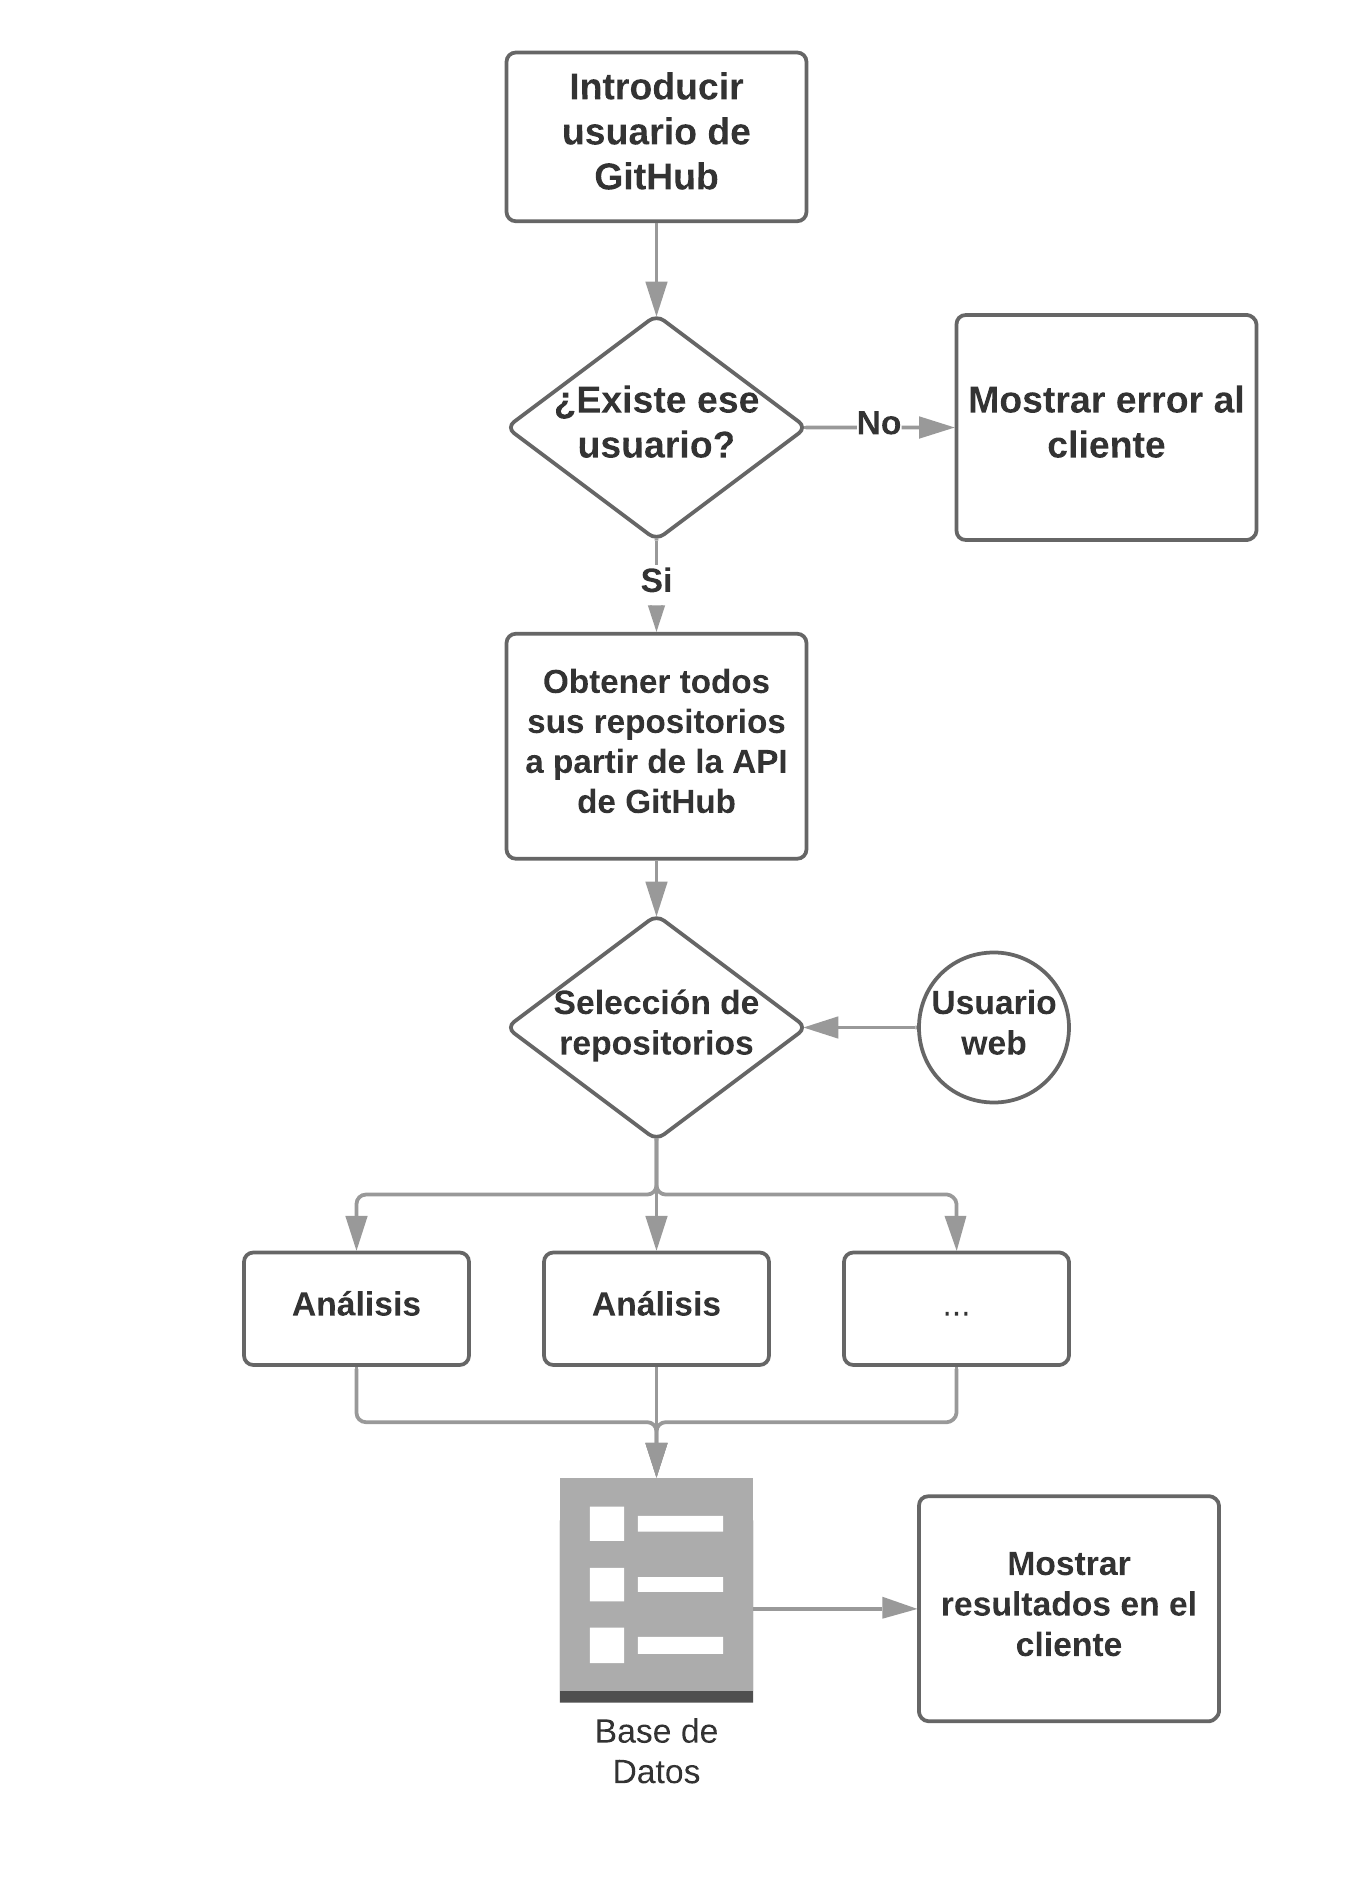
\includegraphics{img/pedir_repos_user.png}
    \caption{Gráfico de petición de análisis de un usuario}
    \label{fig:oneuser}
\end{figure}

La primera etapa del análisis es la introducción de un usuario u organización de GitHub para realizar el análisis de sus repositorios. Otra opción más simplificada sería el análisis de un único repositorio, que simplificaría la explicación del proceso. En la figura \ref{fig:inicio} se puede ver la página de inicio. 

\begin{figure}
    \centering
    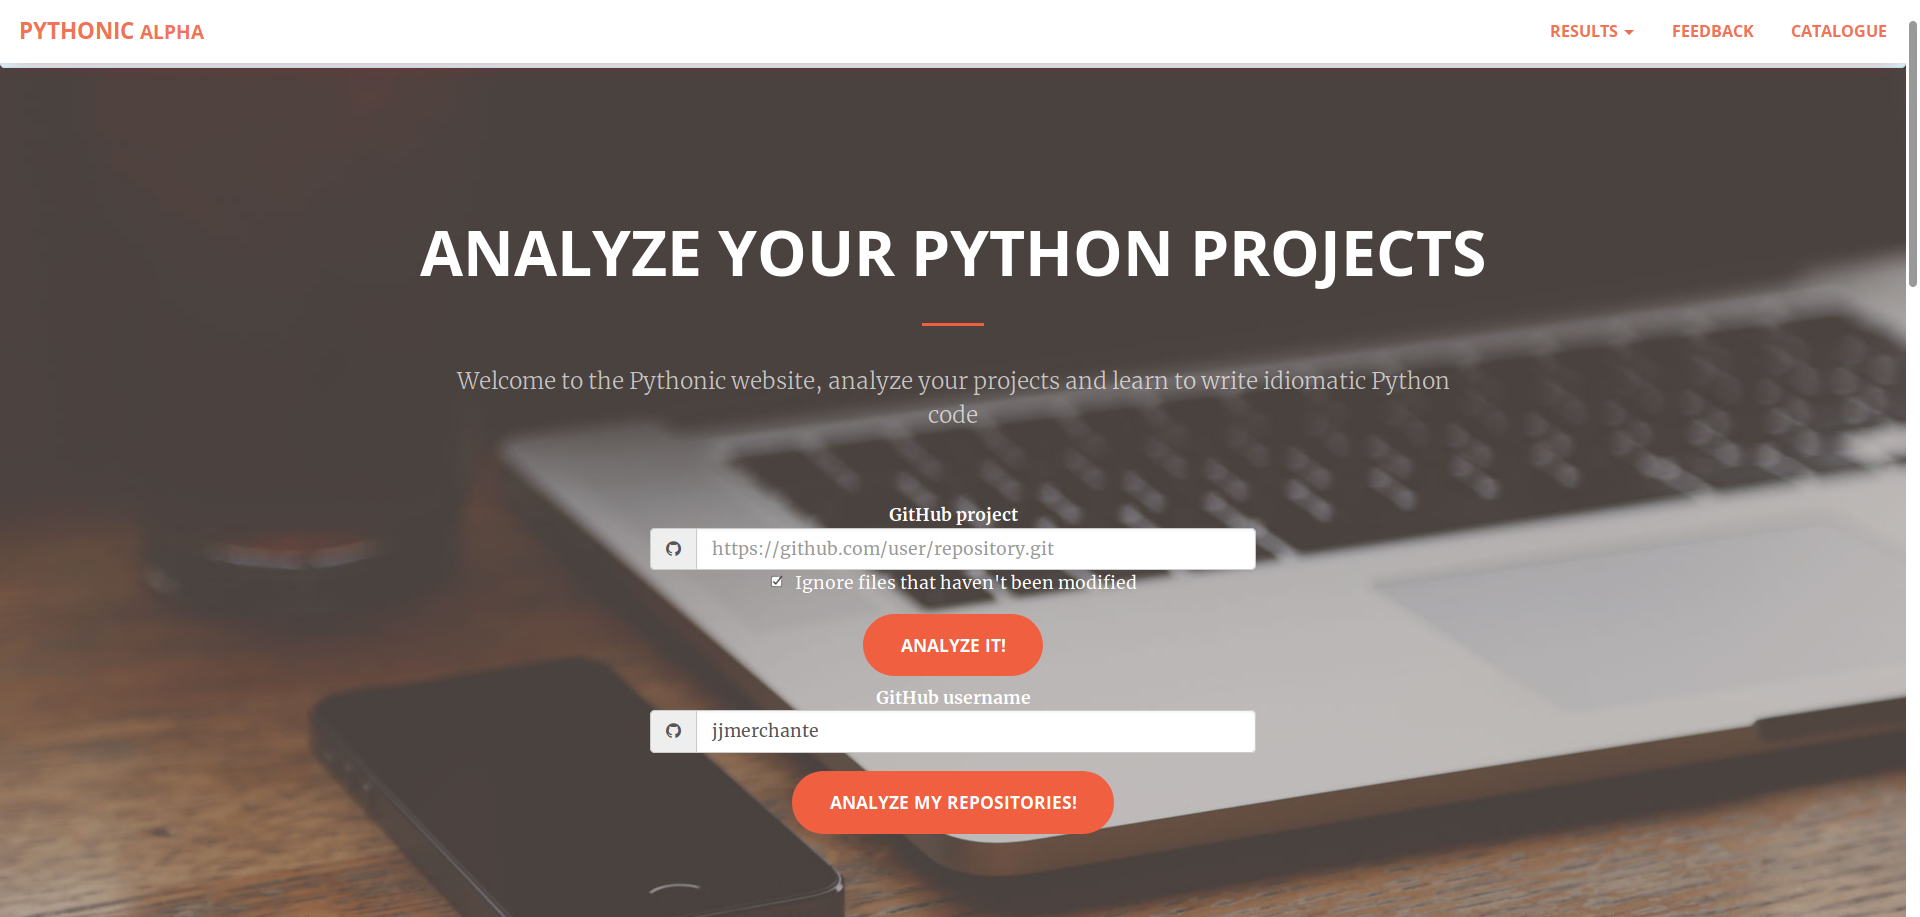
\includegraphics[width=0.9\textwidth]{img/1inicio.png}
    \caption{Página principal}
    \label{fig:inicio}
\end{figure}

Una vez introducido el usuario, el navegador realizará una consulta al servidor Django para obtener todo los repositorios de la cuenta del usuario. 

\texttt{GET /repos-user/<name>}

Django realizará una consulta a la API de GitHub para recabar información. Obtendrá el listado de los repositorios del usuario, y por cada uno de ellos el lenguaje principalmente utilizado y conocer si es un \textit{fork}(una copia del repositorio de otro usuario).

\texttt{GET https://api.github.com/users/<name>/repos}

Toda la información obtenido se mostrará en el navegador, para que de esta manera se pueda seleccionar los repositorios que quiere que se analicen. Por poner un ejemplo, si un usuario sabe que no hay código de Python en un determinado repositorio, no tendría sentido seleccionarlo. Además se le ofrece la opción al usuario de indicar otros repositorios a los que ha contribuido para hacer el análisis más preciso. Un ejemplo gráfico se muestra en la figura \ref{fig:pediruser}

\begin{figure}
    \centering
    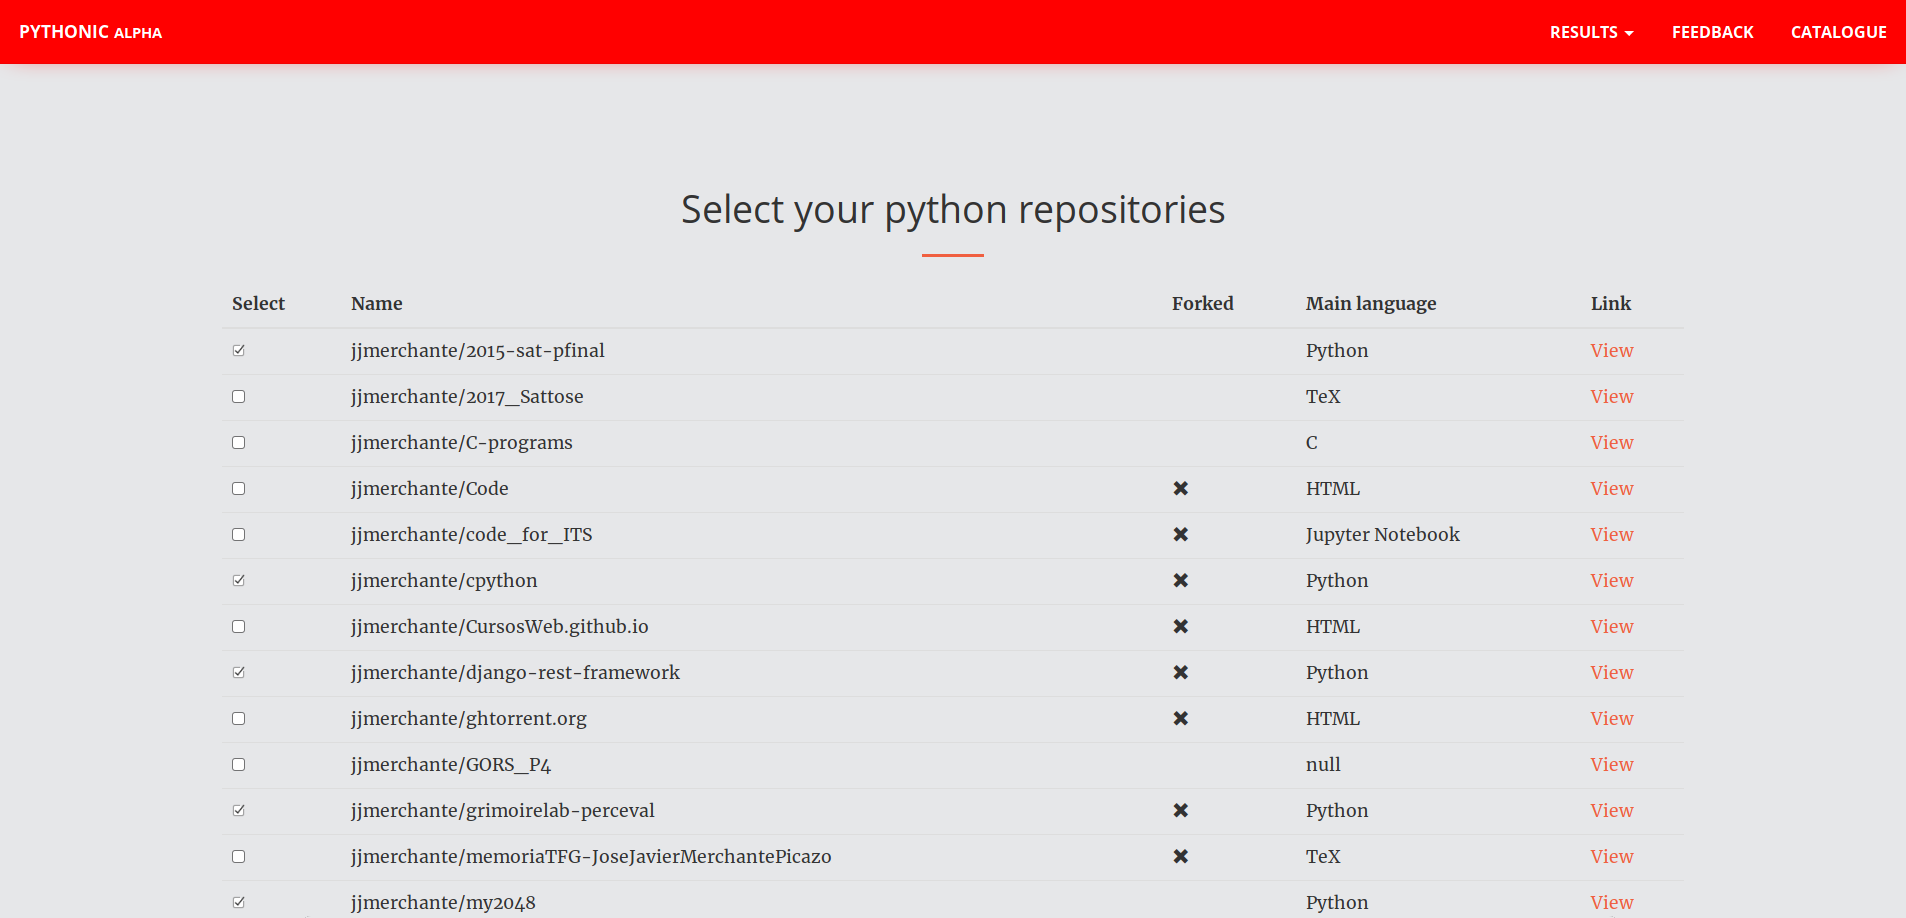
\includegraphics[width=0.9\textwidth]{img/1seleccionar.png}
    \caption{Selección de repositorios}
    \label{fig:pediruser}
\end{figure}

Cuando el usuario tiene decididos los repositorios que se van a analizar, envía los datos al servidor. 

\texttt{POST /analyze-repos-user}\\
\texttt{repos: ["https://github.com/abc/cde.git", ...] username: <name>}

Cada análisis se crea en un thread separado, y cada uno se encarga de publicar su estado en una base de datos cada cierta cantidad de datos analizados.

Los resultados de cada \textit{idiom} se almacena en la base datos con el formato de la tabla \ref{table:result}:


\begin{table}[H]
\begin{center}
\begin{tabular} { | l | l | }
\hline
\textbf{Campo} & \textbf{Valor} \\
\hline
repository &  ForeignKey \\ 
idiomName &  CharField \\ 
line &  IntegerField \\ 
file &  CharField \\ 
author & EmailField \\ 
method &  CharField \\ 

\hline
\end{tabular}
\end{center}
\caption{Tabla de resultados en la base de datos}
\label{table:result}
\end{table}


En la interfaz web del navegador se muestra en todo momento el progreso de cada uno de los repositorios tal y como se observa en la figura \ref{fig:usuario}. 

\begin{figure}[H]
    \centering
    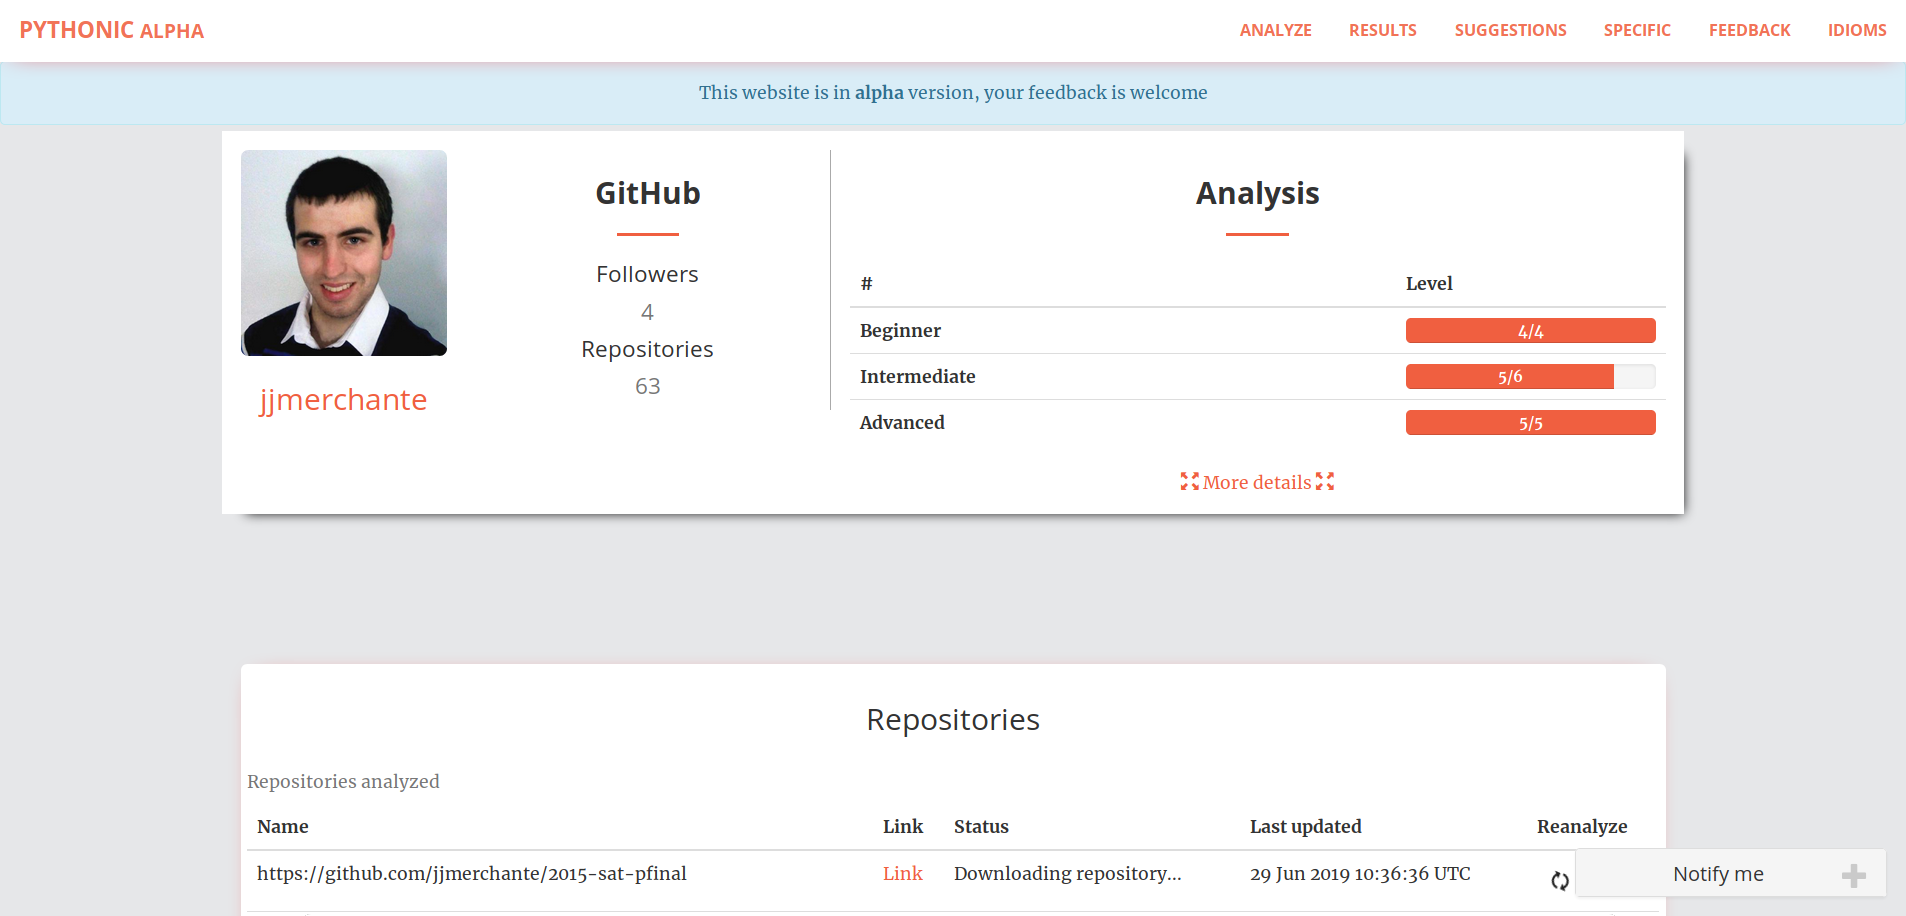
\includegraphics[width=0.9\textwidth]{img/1usuario.png}
    \caption{Resultados de un usuario}
    \label{fig:usuario}
\end{figure}

Cada vez se analiza un proyecto, el usuario puede acceder a la información del repositorio para ver todos los \textit{idioms} que han sido encontrados. Una demostración visual se encuentra en la figura \ref{fig:resultrepo}

\begin{figure}[H]
    \centering
    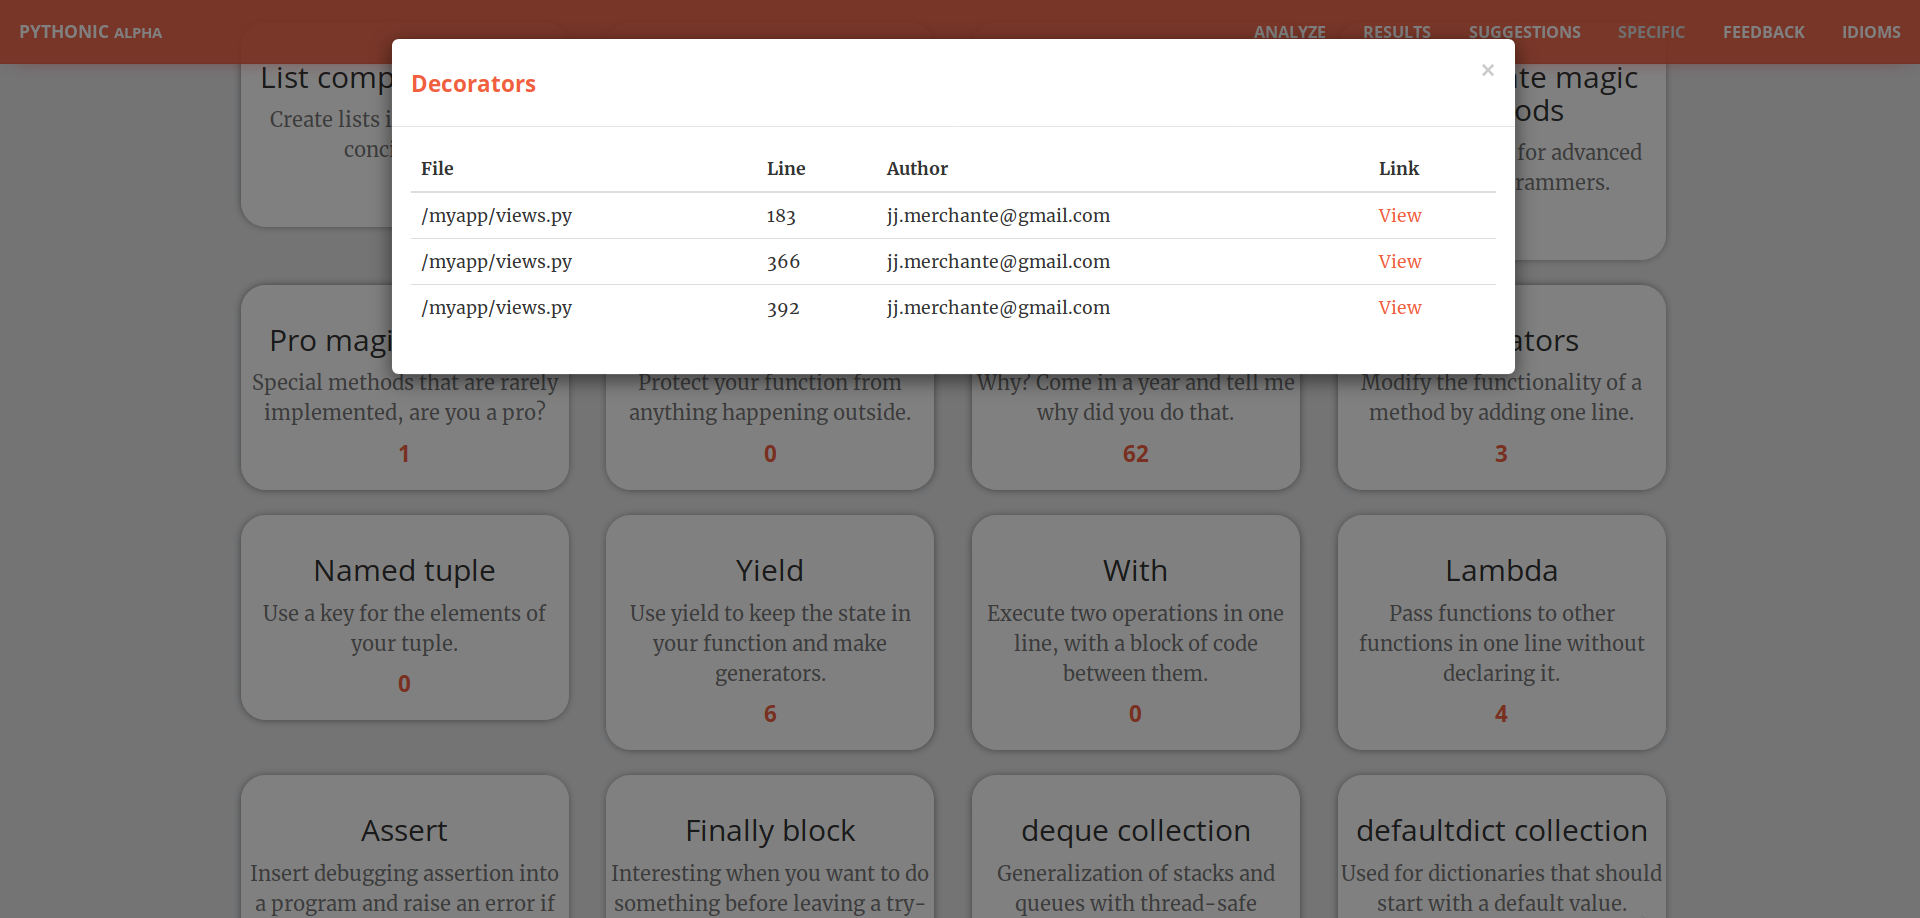
\includegraphics[width=0.9\textwidth]{img/1result_Repo2.png}
    \caption{Resultados de un repositorio. Indica la localización de cada \textit{idiom}}
    \label{fig:resultrepo}
\end{figure}

En ocasiones, el análisis de algunos repositorios puede ser lento debido a la cantidad de ficheros para analizar, para ese tipo de casos, en la interfaz web se ha incorporado la posibilidad de notificar al usuario mediante correo electrónico.

Por otro lado, en la página del usuario analizado, se intentan mostrar sus propios \textit{idioms}. El manejo de identidades, en este caso, es bastante mínimo pero funcional para muchas situaciones.

Por cada uno de los \textit{idioms} encontrados podemos conocer el autor de la línea con \textit{git blame} y a partir de ahí obtener el correo electrónico. 

El \textit{mail} de un usuario es algo más complicado de obtener. En la mayoría de los casos no se indica su correo electrónico de manera pública, por lo tanto nos limita.

Sin embargo, podemos acceder a su historial de \textit{commits} (tiene un alcance limitado y si no ha tenido actividad durante el último mes es probable que no se reflejen resultados) y a partir de ahí se puede obtener su correo electrónico para cruzar los datos e indicar cuáles eran sus \textit{idioms}.

Conociendo los \textit{idioms} que utiliza un usuario en su código, podemos saber cuáles no utiliza, de esta manera, podemos ofrecerle documentación acerca de nuevos elementos \textit{pythonic} que podrían serle de gran utilidad para aprender.

\section{Recopilación de \textit{idioms} con ejemplos}

Finalmente, en la misma página web se incluye un apartado con un catálogo de \textit{pythonic idioms} que hemos considerado de mayor relevancia para mostrar a los usuarios.

Esta selección de elementos y estructuras, incluye una variedad de ejemplo para ilustrar cuándo deben usarse con referencias externas para ampliar la documentación.

Las categorías en las que hemos divido los \textit{idioms} han sido por legibilidad y por rendimiento, mostrando ejemplos en ambos casos.

La lista completa de \textit{idioms} incluidos son los siguientes:
\begin{itemize}
    \item \textit{List comprehensions}: manera concisa de realizar lista en una única linea a partir de otras secuencias
    \item \textit{Dict comprehensions}: forma elegante de construir un diccionario de manera similar a las \textit{list comprehensions}
    \item \textit{Decorators}: permite modificar el comportamiento de una función sin alterar su código
    \item \textit{Magic methods}: son métodos especiales que pueden ser utilizados al usar determinada sintaxis en Python.
    \item \textit{Finally}: permite ejecutar código cuando finalice un bloque. Es común en otros lenguajes.
    \item \textit{Context manager}: con \textit{with} se pueden ejecutar un bloque de código con unas condiciones de inicio y fin. Por ejemplo útil para la apertura de ficheros.
    \item \textit{enumerate}: dado un objeto iterable devuelve una tupla con el índice de cada elemento y el valor.
    \item \textit{Generators}: permite la utilización de funciones como generadores de contenido sin la necesidad de mantener la información que se genera en memoria.
    \item \textit{Generator expressions}: forma concisa de crear generadores similares a las \textit{list comprehensions}.
    \item \textit{defaultdict}: misma funcionalidad que la de un diccionario con la peculiaridad de que se puede definir un valor por defecto para los elementos que no están creados.
    \item \textit{deque}: es una cola en ambos sentidos (cola y pila)
    \item \textit{counter}: es una subclase del diccionario que permite contar objetos.
    \item \textit{classmethod}: indica que el método pertenece a la clase. No necesita una instancia para ser llamado.
    \item \textit{staticmethod}: no recibe la clase como parámetro al contrario que \textit{classmethod}, ``no tiene'' referencias a las clase.
    \item \textit{zip}: permite agrupar elementos a partir de dos secuencias diferentes.
    \item \textit{itertools}: una serie de funciones que permite operar sobre iteradores.
    \item \textit{total\_ordering}: definiendo un método para ``=='' y uno diferente de comparación, permite suplir el resto para una determinada clase.
\end{itemize}

En la figura \ref{fig:ejemploidiom} muestra el formato con el que se representan los ejemplos.
\begin{figure}[H]
    \centering
    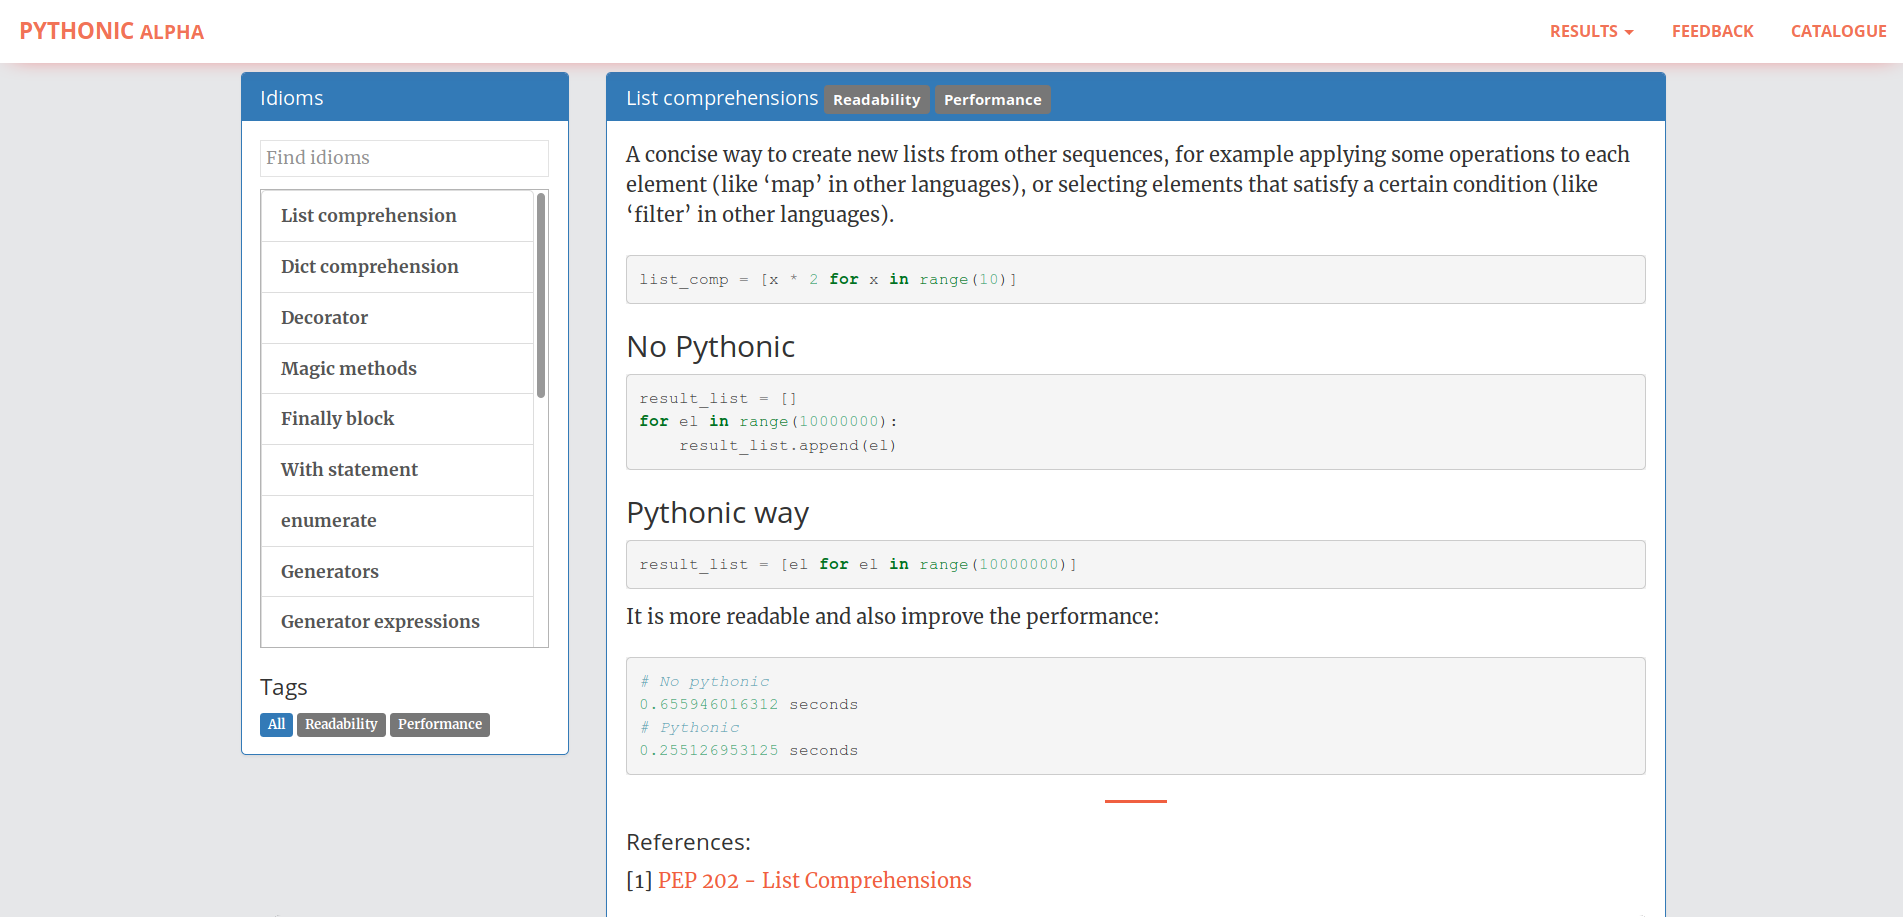
\includegraphics[width=0.9\textwidth]{img/1idioms.png}
    \caption{Explicación de \textit{list comprehension} en la web}
    \label{fig:ejemploidiom}
\end{figure}

%%%%%%%%%%%%%%%%%%%%%%%%%%%%%%%%%%%%%%%%%%%%%%%%%%%%%%%%%%%%%%%%%%%%%%%%%%%%%%%%
%%%%%%%%%%%%%%%%%%%%%%%%%%%%%%%%%%%%%%%%%%%%%%%%%%%%%%%%%%%%%%%%%%%%%%%%%%%%%%%%
% CONCLUSIONES %
%%%%%%%%%%%%%%%%%%%%%%%%%%%%%%%%%%%%%%%%%%%%%%%%%%%%%%%%%%%%%%%%%%%%%%%%%%%%%%%%

\cleardoublepage
\chapter{Conclusiones}
\label{chap:conclusiones}

En este capítulo se indican las conclusiones y resultados finales obtenidos tras la realización de este proyecto. La consecución de los objetivos ha sido prácticamente total. No obstante, siempre existe un determinado margen de mejora sobre el que se puede hacer un estudio intenso. En este apartado además se mencionan lecciones aprendidas a lo largo del proyecto y se concluye con una valoración personal acerca del desarrollo del mismo.

\section{Consecución de objetivos}
\label{sec:consecucion-objetivos}

Como en todo proyecto es siempre importante analizar con detalle qué logros han sido conseguidos y analizar el desarrollo del trabajo realizado. Por todo ello, es importante debatir los objetivos logrados del Capítulo 2 de manera objetiva.

Este proyecto se divide en dos partes principalmente diferenciadas. Por un lado se encuentra la realización de entrevistas a programadores de Python con el objetivo principal de recabar información acerca del lenguaje.

Las entrevistas fueron realizadas a trece candidatos, en principio el número puede parecer escaso, sin embargo, atendiendo a la variedad de perfiles, y a la correlación entre ellos, parece también justo afirmar que las conclusiones obtenidas podrían haber sido bastante similares de tener un mayor número de candidatos.

Las respuestas obtenidas, atendiendo a los objetivos, nos dieron una idea bastante precisa acerca de qué opina la comunidad que programa con Python acerca de los elementos \textit{pythonic}. Suelen considerarlos estructuras que demuestran la madurez de un programador en el lenguaje, suelen facilitar la lectura del código y en algunas ocasiones mejoran el rendimiento del mismo.

Por otro lado, hemos notado cómo la importancia que dan para las empresas que publican su código en abierto al código \textit{pythonic} es superior a las empresas en código cerrado, no obstante, quizá es una opinión sesgada, debido a que la mayor parte de candidatos publicaban su código.

La manera en que se transmiten los \textit{idioms} por la comunidad tiende a ser variada, principalmente es leyendo código de otros programadores, sin embargo, en muchas ocasiones es el interés que despierta el lenguaje. En Python, siempre existe una manera buena de hacer las cosas~\cite{peters2010zen}, por lo tanto, aprender esa metodología siempre te va a hacer mejor programador.

En la parte del servicio web, siento haber conseguido integrar el software de mi TFG para que en este caso fuera más accesible para cualquier usuario. Ofrecer datos más enriquecidos siempre motiva más al usuario final.

Por otro lado incluir un catálogo de \textit{idioms} a la web me pareció un acierto debido a que integra el aprendizaje en un único lugar.

No obstante, hubo una parte que no logré integrar a la perfección. El análisis de \textit{anti-idioms} y la detección de los mismos. Podría considerarse como una mejora del mismo para ofrecer un mayor nivel de análisis de repositorios. Por el momento la web es un método de aprendizaje, quizá la detección de \textit{anti-patrones} pueda incorporarse en mejor medida en un IDE donde el usuario puede identificar la mejora en tiempo real, y no tras subir su código a un repositorio.

En definitiva, prácticamente todos los objetivos propuestos al inicio de este proyecto han sido abordados y superados con éxito.


\section{Lecciones aprendidas}
\label{sec:lecciones_aprendidas}

A lo largo del proyecto, he podido adquirir nuevos conocimientos y experiencias que no se imparten directamente en el máster. 
La realización de entrevistas puede parecer algo relacionado más directamente con carreras de ciencias sociales, en cambio, leyendo documentación y artículos, he podido comprobar que existe una gran cantidad de proyectos, sobre todo de investigación, que precisan de una parte más social.

Preguntar a un determinado colectivo te aporta una gran información, que quizá buscando en la web puede parecer sesgada por tus búsquedas anteriores. Así mismo la realización de entrevistas me ha enseñado que cada entrevista es distinta a la anterior, cada persona puede orientarla hacia su punto de vista a pesar de que las preguntas vayan en un guión.

Por otro lado, en relación a realizar el servicio web, la complicación no fue demasiado elevada, pero siempre te encuentras con problemas de los que acabas aprendiendo un poco más.

Considero importante este trabajo de fin de máster con el que he podido obtener nuevo conocimiento, quizá más enfocado a un ámbito más de investigación, pero que genera una nueva visión en esta nueva etapa


\section{Trabajos futuros}
\label{sec:trabajos_futuros}

Es importante señalar que todo proyecto puede mejorarse, se pueden integrar nuevas funcionalidades o mejorar de cara a un usuario. El estudio de análisis de \textit{idioms} es un campo que tiene mucho recorrido, es por ello que en este epígrafe se señalan algunos puntos para futuros trabajos:
\begin{enumerate}
    \item Podría ser interesante crear un\textit{ plug-in} para un IDE que permita identificar anti-\textit{idioms} y que el usuario pueda detectarlo al momento. De este modo se podría mejorar la legibilidad del código desde el primer momento.
    \item Para la página web podría haber mejoras en relación al manejo de identidades para identificar el autor de un \textit{idiom}. Podrían mostrarse al usuario agrupaciones de correos o nombres para que las pueda relacionar.
    \item Para realizar un mejor estudio de Python se podrían realizar encuestas simples con fragmentos de código para saber qué es lo que consideran más o menos \textit{pythonic}.
    \item Otro posible análisis sería identificar la evolución de \textit{idioms} a lo largo del tiempo sobre una muestra considerable de repositorios con alta actividad durante un largo periodo de tiempo.
\end{enumerate}




%%%%%%%%%%%%%%%%%%%%%%%%%%%%%%%%%%%%%%%%%%%%%%%%%%%%%%%%%%%%%%%%%%%%%%%%%%%%%%%%
%%%%%%%%%%%%%%%%%%%%%%%%%%%%%%%%%%%%%%%%%%%%%%%%%%%%%%%%%%%%%%%%%%%%%%%%%%%%%%%%
% APÉNDICE(S) %
%%%%%%%%%%%%%%%%%%%%%%%%%%%%%%%%%%%%%%%%%%%%%%%%%%%%%%%%%%%%%%%%%%%%%%%%%%%%%%%%

\cleardoublepage
\appendix

\chapter{Preguntas realizadas en las entrevistas}
\label{app:interview_questions}
 Las principales preguntas realizadas a los entrevistados son las que aparecen en la siguiente lista. El orden pudo haber cambiado en dependencia a las respuestas dadas, algunas pudieron ser respondidas previamente y otras fueron espontáneas para conocer algún detalle más en concreto.
 
 \begin{itemize}
     \item ¿Eres familiar con el término \textit{pythonic}? ¿Qué es para ti?
     \item ¿Podrías darnos algún ejemplo?
     \item En tu opinión, ¿el código \textit{pythonic} es importante? ¿Es el concepto de código \textit{pythonic} diferente de la necesidad de un estilo de código en otros lenguajes? ¿Cuáles son las principales diferencias?
     \item ¿Crees que es deseable? ¿Qué características crees que son más importantes? ¿Es un programador más avanzado por el uso de \textit{idioms} de Python?
     \item ¿Crees que escribir código \textit{pythonic} es más un estilo o un conjunto de recetas? ¿Podrían ser catalogados?
     \item ¿Cuando programas piensas en usarlos[\textit{pythonic idioms}] o no piensas acerca de ellos?
     \item ¿Crees que tu código es más \textit{pythonic} con los años? ¿Por qué?
     \item ¿Entendías bien los \textit{idioms} cuando empezaste a aprender? ¿Cuáles te parecieron más complicados? (En algunos casos se mencionaron algunos si no se acordaba de ninguno)
     \item ¿Cómo aprendiste a programar más \textit{pythonic}? (En algunos casos se preguntó detalles acerca de conferencias, StackOverflow, compañeros o libros)
     \item ¿Qué IDE usas habitualmente? ¿Utilizas alguna extensión o librería para Python?
     \item En el trabajo, ¿cómo de recomendable es el código \textit{pythonic}? ¿Es obligatorio o es una elección personal?
     \item ¿Comparas el código con tus compañeros? ¿Os revisáis el código en términos de estilo?
     \item ¿Subes el código a una plataforma de software abierto?
     \item ¿Crees que programar \textit{pythonic} en una entrevista puede resultar beneficioso?
     \item ¿Podrías ser capaz de diferenciar un programador experto de un principiante por su código? ¿Cómo?
     \item Cuando descubres un nuevo \textit{idiom}, ¿adaptas tu antiguo código?
 \end{itemize}

También se mostraron a algunos entrevistados (los que fueron en persona) una lista con una serie de \textit{idioms} para identificar diferentes aspectos para la mejora de la herramienta de detección del nivel de un programador Python.


%%%%%%%%%%%%%%%%%%%%%%%%%%%%%%%%%%%%%%%%%%%%%%%%%%%%%%%%%%%%%%%%%%%%%%%%%%%%%%%%
%%%%%%%%%%%%%%%%%%%%%%%%%%%%%%%%%%%%%%%%%%%%%%%%%%%%%%%%%%%%%%%%%%%%%%%%%%%%%%%%
% BIBLIOGRAFIA %
%%%%%%%%%%%%%%%%%%%%%%%%%%%%%%%%%%%%%%%%%%%%%%%%%%%%%%%%%%%%%%%%%%%%%%%%%%%%%%%%

\cleardoublepage

% Las siguientes dos instrucciones es todo lo que necesitas
% para incluir las citas en la memoria
\bibliographystyle{abbrv}
\bibliography{memoria}  % memoria.bib es el nombre del fichero que contiene
% las referencias bibliográficas. Abre ese fichero y mira el formato que tiene,
% que se conoce como BibTeX. Hay muchos sitios que exportan referencias en
% formato BibTeX. Prueba a buscar en http://scholar.google.com por referencias
% y verás que lo puedes hacer de manera sencilla.
% Más información: 
% http://texblog.org/2014/04/22/using-google-scholar-to-download-bibtex-citations/

\end{document}
